\label{sec:implementation}

\doubletake{} is implemented as a library and can be linked directly to programs, or can be injected into unmodified binaries by setting the \texttt{LD\_PRELOAD} environment variable on Linux.

At startup, \doubletake{} begins a new epoch. The epoch continues until the program issues an \emph{irrevocable} system call (see Section~\ref{sec:syscalls} for details). Before this call is issued, \doubletake{} checks program state for evidence of errors. The details are presented in Section~\ref{sec:applications}.

If no errors are found, \doubletake{} ends the epoch, issues the irrevocable system call, and begins a new epoch. If it has found evidence of an error, \doubletake{} enters re-execution mode. The remainder of this section describes the implementation of \doubletake{}'s core functionality.

\subsection{Epoch Start}
\label{sec:implementation/start}

At the beginning of each epoch, \doubletake{} takes a snapshot of program state. \doubletake{} saves all writable memory (stack, heap, and globals) from the main program and any linked libraries, and saves register state of each thread with the \texttt{getcontext} function. Read-only memory does not need to be saved. To identify all writable mapped memory, \doubletake{} reads the Linux \texttt{/proc/self/map} file. \doubletake{} also saves file positions of all open files. This lets programs issue \texttt{read} and \texttt{write} system calls without ending the current epoch. \doubletake{} uses the saved memory state and file positions to ``undo'' these calls if the epoch needs to be re-executed when an error is found.

%%%%%%%%%%%%%%%%%%%%%%%%%%%

\subsection{Normal Execution}
\label{sec:implementation/normalexecution}

Once a snapshot has been saved, \doubletake{} lets the program execute normally. Most program operations proceed normally, but \doubletake{} interposes on heap allocations and system calls in order to set tripwires and support re-execution.

%%%%%%%%%%%%%%

\subsubsection*{System Calls}
\label{sec:syscalls}
\begin{table}[t]
	\centering
	\small
	\renewcommand{\arraystretch}{1.5}
	\begin{tabular}{l|p{6cm}}
		\textbf{Category} & \textbf{Functions} \\
		\hline
		
		Repeatable		& \texttt{getpid}, \texttt{sleep}, \texttt{pause}\\
		
		Recordable		& \texttt{mmap}, \texttt{gettimeofday}, \texttt{time}, 
						  \texttt{clone} , \texttt{open}\\
		
		Revocable		& \texttt{write}, \texttt{read} \\
		
		Deferrable		& \texttt{close}, \texttt{munmap} \\
		
		Irrevocable		& \texttt{fork}, \texttt{exec}, \texttt{exit}, \texttt{lseek}, \texttt{pipe}, \texttt{flock}, \texttt{socket related system calls}\\
	\end{tabular}
	\caption{System calls handled by \doubletake{}. All unlisted system calls are conservatively treated as irrevocable, and will end the current epoch. Section~\ref{sec:syscalls} describes how \doubletake{} handles calls in each category.\label{table:syscalls}}
\end{table}

\doubletake{} ends each epoch when the program attempts to issue an irrevocable system call. However, most system calls can safely be re-executed or undone prior to re-execution. 

\doubletake{} breaks system calls into five categories, shown in Table~\ref{table:syscalls}. System calls could be intercepted using \texttt{ptrace}, but this would add unacceptable overhead during normal execution. Instead, \doubletake{} interposes on all library functions that may issue system calls.

%%%%%%%

\emph{Repeatable system calls} do not modify system state, and return the same result during normal execution and re-execution. No special handling is required for these calls.

\begin{figure*}[ht!]
	\begin{center}
		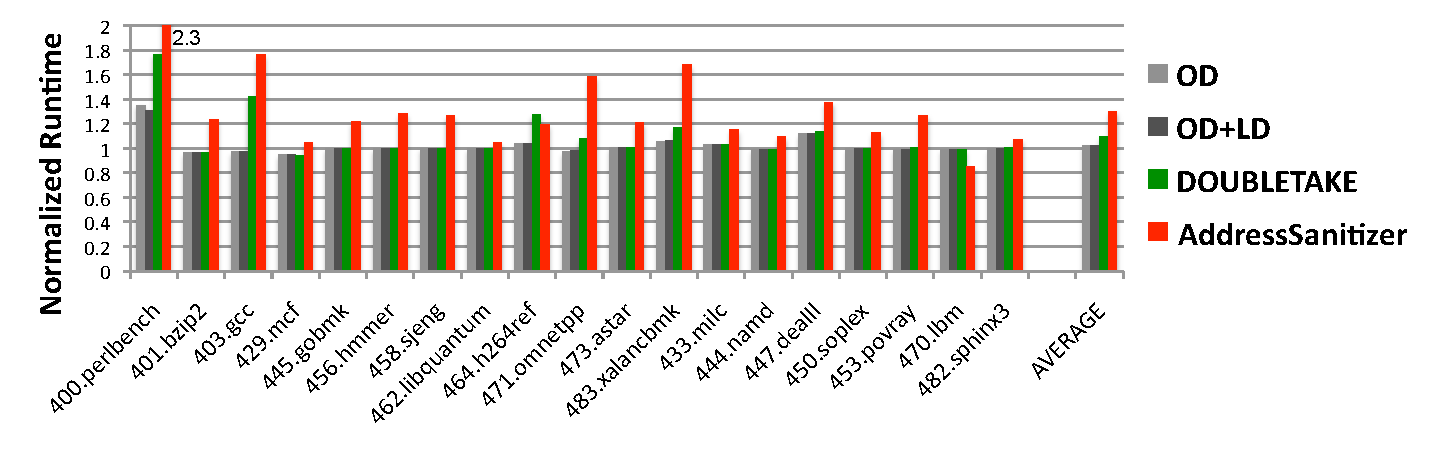
\includegraphics[width=6.5in]{figure/perf}
	\end{center}
	\caption{Runtime overhead of \doubletake{} (OD = Buffer Overflow Detection, LD = Leak Detection, \doubletake{} = all three detections enabled) and AddressSanitizer, normalized to each benchmark's original execution time. 
%Overhead for Valgrind is reported in Table~\ref{table:valgrind} because the results do not fit on this graph.
\label{fig:perf}}
\end{figure*}

%%%%%%%

\emph{Recordable system calls} may return different results if they are re-executed. \doubletake{} records the result of these system calls during normal execution, and returns the saved result during re-execution. Some recordable system calls, such as \texttt{mmap}, change the state of underlying operating system. \CC{\doubletake{} replays the results of \texttt{mmap} in re-execution. It is safe to replay this although the memory maps created by \texttt{mmap} remains mapped even in the beginning of re-execution, which is different with the situation of normal execution; Because there is no memory access on these maps until corresponding \texttt{mmap}s arecalled, otherwise the program can crash in normal execution.}

\emph{Revocable system calls} modify system state, but \doubletake{} can save the original state beforehand and restore it prior to re-execution. Most file I/O fall into this category. For example, \texttt{write} modifies file contents, \doubletake{} can write the same content during re-execution. \texttt{write} also changes the current file position, which \doubletake{} restores to the saved file position using \texttt{lseek} prior to re-execution. \doubletake{} saves all file descriptors of opened files in a hash table at the beginning of each epoch. In addition, \doubletake{} must save stream contents returned by \texttt{fread}. Calls to \texttt{read} and \texttt{write}  on normal files, which can be identified by check the hash map, don't need to be handled. But those calls on socket files are treated as irrevocable system calls.
	
\emph{Deferrable system calls} will irrevocably change program state, but can safely be delayed until the end of the current epoch. \doubletake{} delays all calls to \texttt{munmap} and \texttt{close}, and executes these system calls before exiting or starting a new epoch.
	
\emph{Irrevocable system calls} change internally-visible program state, and cannot be undone. \doubletake{} must end the current epoch before these system calls are allowed to proceed. Note that for \doubletake{}, the meaning of ``irrevocable'' is different from that used in transactional memory systems~\cite{Irrevocabletrans}. Unlike in transactions, we expect re-execution to be identical to the epoch's original execution. It is safe for system calls to affect externally-visible state as long as the effect on internal state can be hidden or undone.

\CC{ REMOVED THIS. First, it is unrelated here and should be putted to multithreading support. : Note that in the presence of multiple threads, an error may fail to appear in the re-execution because of data races (synchronization ordering is already tracked and replayed). \doubletake{} then re-executes the code in an attempt to reveal the error. }

%%%%%%%%%%%%%%

\subsubsection*{Multithreaded Support}
We have implemented support for multiple threads, but the recording and re-execution of thread synchronizations is not yet stable. 

\doubletake{} records the sequence of synchronizations and corresponding results separately for each thread. Basically, a synchronization event is recorded in two lists simultaneously, a per-thread list and a synchronization variable list. 

Every mutex records the order of threads that acquire it, and condition variables record the order of thread wake-ups. \doubletake{} does not enforce a total global order on lock acquisitions. Operations within a single thread are totally-ordered and recorded, and \doubletake{} enforces local order \CC{for each synchronization variable}. In the absence of data races, this is sufficient to ensure deterministic re-execution. If it fails to reveal the error on replay, \doubletake{} has effectively tolerated the error and continues execution.

Calls to \texttt{pthread\_create} are recorded with the same mechanism as recordable system calls. When a new thread starts, \doubletake{} takes a snapshot of the thread's stack and registers to enable re-execution from the beginning of the thread's execution. As with synchronization operations, \doubletake{} logs thread creation order and enforces this order during re-execution.  Threads exits are deferred until the end of the epoch. \texttt{pthread\_join} is effectively deferred as well.

%%%%%%%%%%%%%%

\subsubsection*{Heap Allocator}
\label{sec:heapallocator}

Heap allocators typically issue a large number of \texttt{mmap} or \texttt{sbrk} system calls, which would complicate \doubletake{}'s logging to facilitate re-execution. \doubletake{} replaces the default heap with a fixed-size BiBOP-style allocator with per-thread subheaps and power-of-two size classes, built using Heap Layers~\cite{heaplayers}. 


\doubletake{} uses a separate heap for internal usage and only uses this custom heap allocator for allocations from the application and corresponding libraries. Any additional memory allocations in the replay phase are also allocated from a separate heap too, such as the \texttt{backtrace} call or printing. 

\doubletake{}'s heap is completely deterministic for a program without races, so no logging is required to ensure that allocations do not change during re-execution. To achieve this target, all allocations from the same thread is met at a specific subheap, which obtains every superblock (large chunks of memory) by acquiring a lock. Superblock allocations are deterministic in replay phase, which is enforced by the deterministically acquiring and releasing of a lock. When an object is freed, this object is returned to the current thread issuing this free operation. Because of deterministic superblock allocations and memory free operations (enforced by the program order), we guarantee that all memory allocations are deterministic inside the same subheap. 
 
\doubletake{} keeps information about each heap object in its object header. During allocation, objects are marked as allocated and their \emph{requested size} are saved, which may be less than the power-of-two size class. At deallocation, objects are marked as freed and putted into the quarantine list if the detection of use-after-free is enabled. For non-aligned objects, \doubletake{} also checks buffer overflows for non-aligned words, which can even report one-byte buffer overflows because of exact size. 

\doubletake{} also maintains a bitmap to record the locations of heap canaries. The bitmap records every word of heap memory that contains a canary. \doubletake{} notifies the detection tool when any of the bytes do not contain canaries. Buffer overflow detection places canaries only outside the requested object size. Re-execution is only started if the detection tool finds that canaries between allocated objects have been overwritten.

During replay, \doubletake{}'s heap allocator checks to see if the object being allocated or freed contains the address where an error was detected. If so, \doubletake{} calls the \texttt{backtrace()} function to obtain a call stack for the allocation and deallocation sites. 
%%%%%%%%%%%%%%

\subsubsection*{Epoch End}

The epoch ends when any thread issues an irrevocable system call. All other threads are notified with a signal SIGUSR2. Once all threads have stopped, \doubletake{} checks the program state for errors. The application-specific error checks are described in Section~\ref{sec:applications}. If an error is found, \doubletake{} immediately switches to re-execution mode. If not, the runtime issues any deferred system calls and clears the logs for all recorded system calls.

%%%%%%%%%%%%%%%%%%%%%%%%%%%

\subsection{Rollback}

Before re-executing the current epoch, \doubletake{} must roll back the program state. 

Restoring the saved stack may corrupt the current stack, so \doubletake{} switches to a temporary stack during rollback. The saved state of all writable memory is copied back, and revocable system calls are undone by calling \texttt{lseek} to reset all opening files positions. Then \doubletake{} installs watchpoints before calling \texttt{setcontext} to restore its context. 

Debug registers are not accessible in user-mode, so \doubletake{} must use \texttt{ptrace} to set watchpoints. \doubletake{} forks a child process and attaches to it using \texttt{ptrace} to load watched addresses into the debug registers and enable the watchpoints.

Once watchpoints have been placed, \doubletake{} uses the \texttt{setcontext} call to restore register state and begin re-execution. 

\subsection{Re-Execution}
\label{sec:implementation/re-execution}

During re-execution, \doubletake{} replays the saved results of recordable system calls from the log collected during normal execution. All deferred system calls are converted to no-ops while the program is re-executing. \doubletake{} issues other system calls normally. 

\subsubsection*{Synchronization Replay}
\CC{All New}
\doubletake{} enforces the recorded order of synchronization operations during re-execution by using the {\it semaphore replay} mechanism~\cite{TERN}. \doubletake{} assigns a binary semaphore for each thread, initialized as unavailable. Lock acquisitions and conditional wakeups are treated similarly here. 

Before the rollback, \doubletake{} checks the first synchronization event of every synchronization variable list. If an synchornization event is also the first event of a thread, the semaphore of this thread is incremented immediately. Otherwise, this thread are granted with a pending increment, incremented only after all previous synchronizations of this thread has been  handled.  

In the replay, a lock acquiring is turned into a semaphore wait. During a lock release, \doubletake{} actually increments  the semaphore of next thread in the same synchronization variable list, no matter whether the next thread is the same thread or not. In order to support multiple locks for a critical section, a lock acquisition also increments pending increments if possible. 

\subsubsection{Trap Handler}
\doubletake{} handles traps caused by accesses on watchpoints.  Inside the trap handler, \doubletake{} firstly determines which watchpoint causes the current trap if the fault instruction is not issued from \doubletake{} library. Normally, the debug status register has to be accessed in order to know this information. However, using \texttt{ptrace} is very inconvenient inside a signal handler because of involving in another process. \doubletake{} always keeps an updated value for every watchpoint. Thus, it can precisely determine which watchpoint is triggered by checking the changes of those watchpoints. Also, \doubletake{} prints callsite information of buffer overflows or use-after-free errors and their memory allocation (or deallocation). 







